\chapter{Data Description}
\label{chapterlabel3}
We provide a summary of the way that spatial data is stored in OSM, to give context to the analysis and interpretation of results that will be provided in subsequent chapters.

The data for this analysis was collected from OSM history extract files. While OSM is most often consumed as a user-facing map, it primarily functions as a geospatial database. The OSM data model uses nodes, ways, and relations to represent the geometry of all geographic features \parencite{noauthor_elements_2020}. Nodes commonly represent point features, such as shops, healthcare facilities, and bus stops. Ways are ordered collections of nodes, commonly used to represent features such as roads. Closed ways (where the start and end node are the same) are used to represent areal features, such as buildings. Relations are the least common element, used to represent relationships between multiple data elements. Relations can take many forms, but may, for example, be used describe turn restrictions between road sections \parencite{noauthor_elements_2020}. 

The attributes for all OSM elements are stored using tags, which consist of text key, value pairs. An element can have multiple tags, however each key for a single elements must be unique \parencite{noauthor_tags_2020}. While OSM does not impose any restrictions on the contents of a tag (aside from being a 255-character Unicode string), it is a best-practice within the community to follow established tagging conventions for commonly occurring elements \parencite{noauthor_tags_2020}. For example, the \texttt{highway=residential} tag is used to describe roads that provide access to homes \parencite{noauthor_elements_2020}. The Taginfo website\footnote{\url{https://taginfo.openstreetmap.org/}} allows one to see commonly used tags across the world. Each OSM element also contains metadata such as the timestamp of last edit, version number, and user ID of the contributor \parencite{noauthor_elements_2020}. 

OSM data is commonly downloaded from services such as Geofabrik\footnote{\url{https://www.geofabrik.de/}} or Planet OSM\footnote{\url{https://planet.osm.org/}} in SHP, PBF, or OSM XML format \parencite{mooney_accessing_2011}. An example of the OSM XML format can be found on the relevant OSM Wiki page \parencite{noauthor_osm_2017}. From these services, one can download a copy of the database for the full planet, or from selected continents or countries. This files are usually frequently updated (eg. daily, in the case of Geofabrik) to ensure that new contributions or edits to OSM are reflected in the downloadable data. One can download both current snapshots and full historical OSM data from these services. The historical data provides access to all edits that were ever made in OSM and can allow one to understand various aspects of how the map has matured over time \parencite{corcoran_analysing_2013, mooney_characteristics_2012}. Researchers are able to understand the evolution of individual features in the map, as each feature has an associated version number that allows one to track all revisions \parencite{noauthor_elements_2020}. 

Analyzing historical OSM data has traditionally been challenging, in part due to the incredibly large file size \parencite{raifer_oshdb_2019, mooney_accessing_2011}. The processing described in \textcite{mooney_characteristics_2012}, for example, took 305h. At the time of writing, the full history planet OSM XML file is 140 GB, which is too large for many users or researchers to manage effectively without significant technical expertise. As is surveyed by \textcite{raifer_oshdb_2019}, researchers and practitioners have developed numerous tools and algorithms that allow for simpler processing and querying of this large historical dataset. Examples include the \textit{Is OSM Up-To-Date?} website developed by \textcite{minghini_open_2018}, and the \textit{OSMatrix} website developed by \textcite{roick_technical_2012}. 

The current state-of-the-art in this domain is the recently developed OSHDB framework, which provides a flexible and fast way to perform spatio-temporal analyses on historical OSM data \parencite{raifer_oshdb_2019}. The OSHDB framework allows for the extracted historical OSM data to be stored in any JDBC (Java database connectivity) compliant database system and accessed through an API \parencite{raifer_oshdb_2019}. A custom data model was also developed to allow for more efficient access and parallel processing, as is shown in Figure \ref{fig:oshdb}. Each version of an OSM Entity is grouped by a common ID into a parent OSH Entity. Each OSH Entity has a type that corresponds to one of the OSM data types (nodes, ways, or relations) \parencite{raifer_oshdb_2019}. Application of the OSHD framework for this analysis will be described in the following chapter.

%%%%%%%%%%%%%%%%%%%%%%%%%% DATA MODEL IMAGE 
\begin{figure} % opens the figure environment. the '[H]' forces the image to be Here
    \centering % puts the image in the horizontal centre of the page
    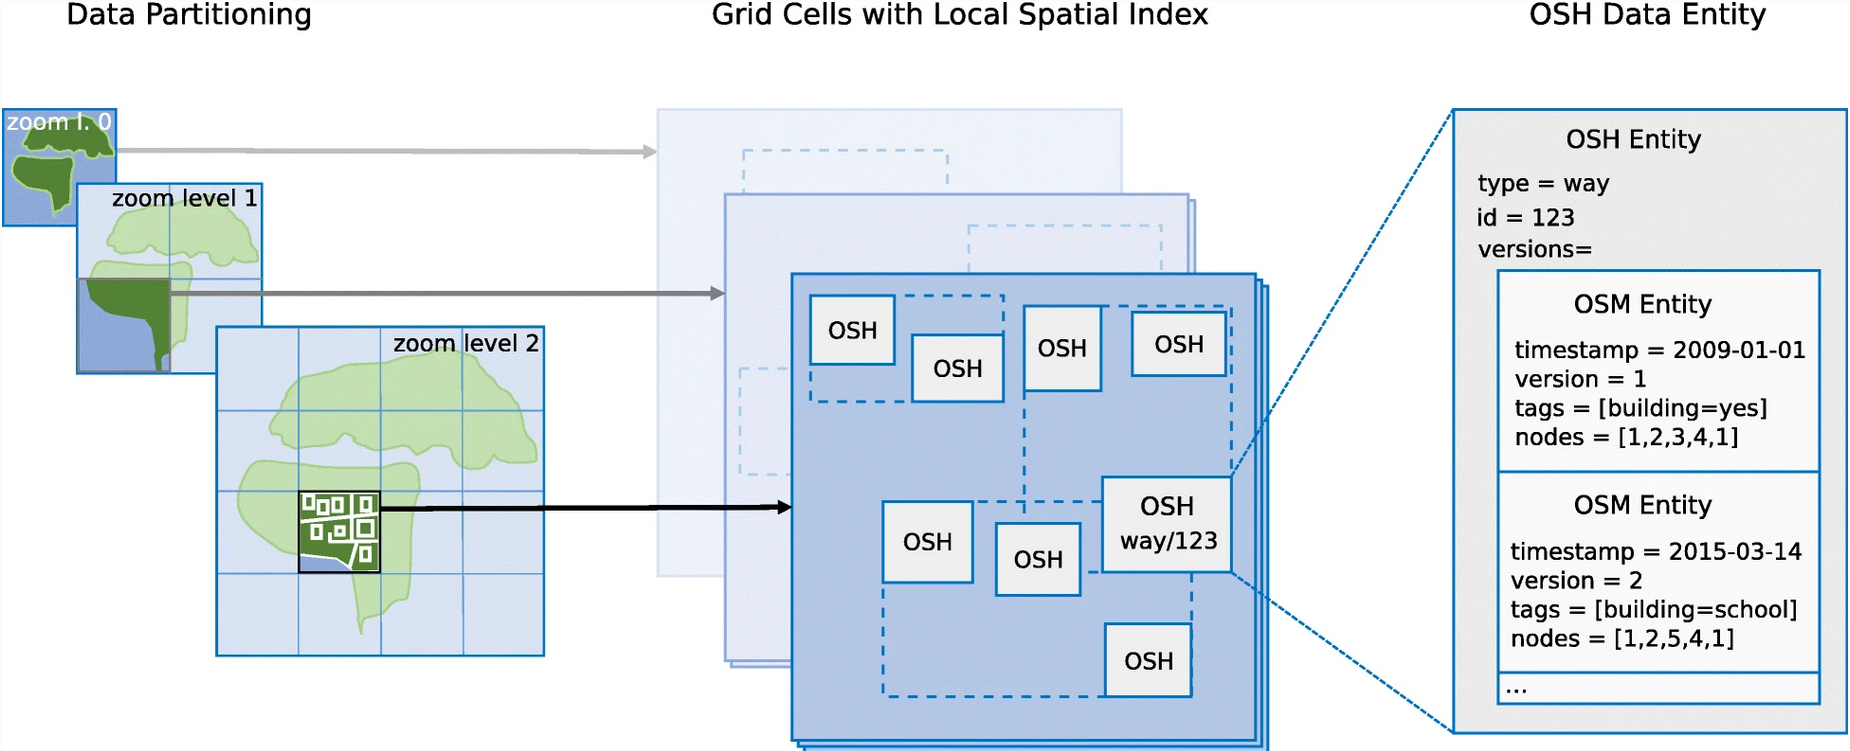
\includegraphics[width = \textwidth]{Images/oshdb.PNG} %this tells latex what graphics to include. 
    \caption{Summary of the OSHDB data model, provided by \textcite{raifer_oshdb_2019}.} % this prints the caption below the figure
    \label{fig:oshdb} % this internally labels the figure for future referencing.
\end{figure}
%%%%%%%%%%%%%%%%%%%%%%%%%% 




    


